
\chapter{Resultados y Discusión}
\label{chap:resultados}

\section{Resultados}
\label{sec:resultados}

\subsection{Comparativa general de modelos}
\label{subsec:comparativa-modelos}

\begin{table}[htbp]
\centering
\scriptsize
\begin{tabular}{p{0.26\textwidth}p{0.17\textwidth}rrrr}
\toprule
Modelo & Entrenamiento & MAE test & RMSE test & \(R^2\) test \\
\midrule
Regresión lineal & estándar & 0.067585 & 0.183824 & 0.096059  \\
Random Forest & estándar & 0.054366 & 0.088403 & 0.790941  \\
XGBoost & estándar & 0.054604 & 0.091735 & 0.774885  \\
Red neuronal secuencial & estándar & 0.055425 & 0.113506 & 0.655354  \\
Quantum Inspired NN & estándar & 0.056056 & 0.143025 & 0.452787  \\
\bottomrule
\end{tabular}
\caption{Comparación final de modelos.}
\label{tab:resultados-modelos}
\end{table}

La Tabla~\ref{tab:resultados-modelos} muestra que las familias de árboles dominan el test. Random Forest estándar obtiene el menor RMSE y el mayor \(R^2\); XGBoost estándar queda cerca, pero con RMSE ligeramente superior. Las redes neuronales no superan a las familias de árboles en esta muestra, aunque la variante Quantum Inspired mejora claramente al aplicar progressive ATM frente a su versión estándar.


\subsection{Entrenamiento estándar frente a progressive ATM}
\label{subsec:normal-vs-progressive}

\begin{table}[htbp]
\centering
\small
\begin{tabularx}{\textwidth}{p{0.22\textwidth}rrr>{\raggedright\arraybackslash}X}
\toprule
Familia & RMSE & RMSE ATM & \(\Delta\) & Lectura \\
\midrule
Regresión lineal & 0.183824 & 0.187747 & +0.003923 & Empeora levemente. \\
Random Forest & 0.088403 & 0.088533 & +0.000130 & Prácticamente neutro. \\
XGBoost & 0.091735 & 0.113606 & +0.021871 & Degrada test. \\
Red neuronal secuencial & 0.113506 & 0.120161 & +0.006655 & Degrada test. \\
Quantum Inspired NN & 0.143025 & 0.117404 & -0.025621 & Mejora clara. \\
\bottomrule
\end{tabularx}
\caption{Impacto agregado de progressive ATM frente a entrenamiento estándar.}
\label{tab:progressive-segmentos}
\end{table}

El entrenamiento progressive ATM no produce una mejora universal. En Random Forest, que ya muestra un comportamiento muy estable en la comparación, el cambio es casi neutro; en XGBoost y en la red secuencial empeora el RMSE test; en Quantum Inspired sí actúa como regularizador útil. Esto encaja con la interpretación metodológica: ordenar por cercanía a ATM puede estabilizar arquitecturas iterativas más sensibles, pero también puede sesgar el aprendizaje si los extremos de moneyness contienen información necesaria para test. Por tanto, progressive ATM debe tratarse como variante experimental y no como decisión automática.

La evidencia sugiere una lectura por familias.

\begin{itemize}
  \item En \textbf{Random Forest}, la proximidad de resultados indica que el bosque ya capta bien la señal central sin necesitar entrenamiento progresivo ATM.
  \item En \textbf{XGBoost} y en la \textbf{red secuencial}, el deterioro sugiere que priorizar ATM puede dejar peor representadas zonas relevantes para la generalización final.
  \item En \textbf{Quantum Inspired}, la mejora apunta a que la estrategia sí puede actuar como regularizador estructural cuando la arquitectura es más sensible al orden de aprendizaje.
\end{itemize}

La conclusión práctica es sobria: progressive ATM es útil como hipótesis de trabajo y como herramienta de análisis, pero su activación debe justificarse por evidencia empírica en cada familia concreta. Se puede ver más en el apéndice \ref{app:progressive}.

\subsection{Modelo de referencia}
\label{subsec:modelo-final}

El modelo de referencia es el XGBoost:
\begin{itemize}
    \item Desempeño en test muy notable quedando muy cercano al mejor desempeño entre todas las familias.
    \item Los modelos de regresión simbólica y árboles de decisión consiguen explicar el modelo mejor que al resto de familias: $RMSE=0.0378$, $MAE=0.0219$, $R2=0.9264$
\end{itemize}

\subsection{Diagnóstico de rendimiento}
\label{subsec:diagnostico-rendimiento}


\begin{figure}[!htbp]
\centering
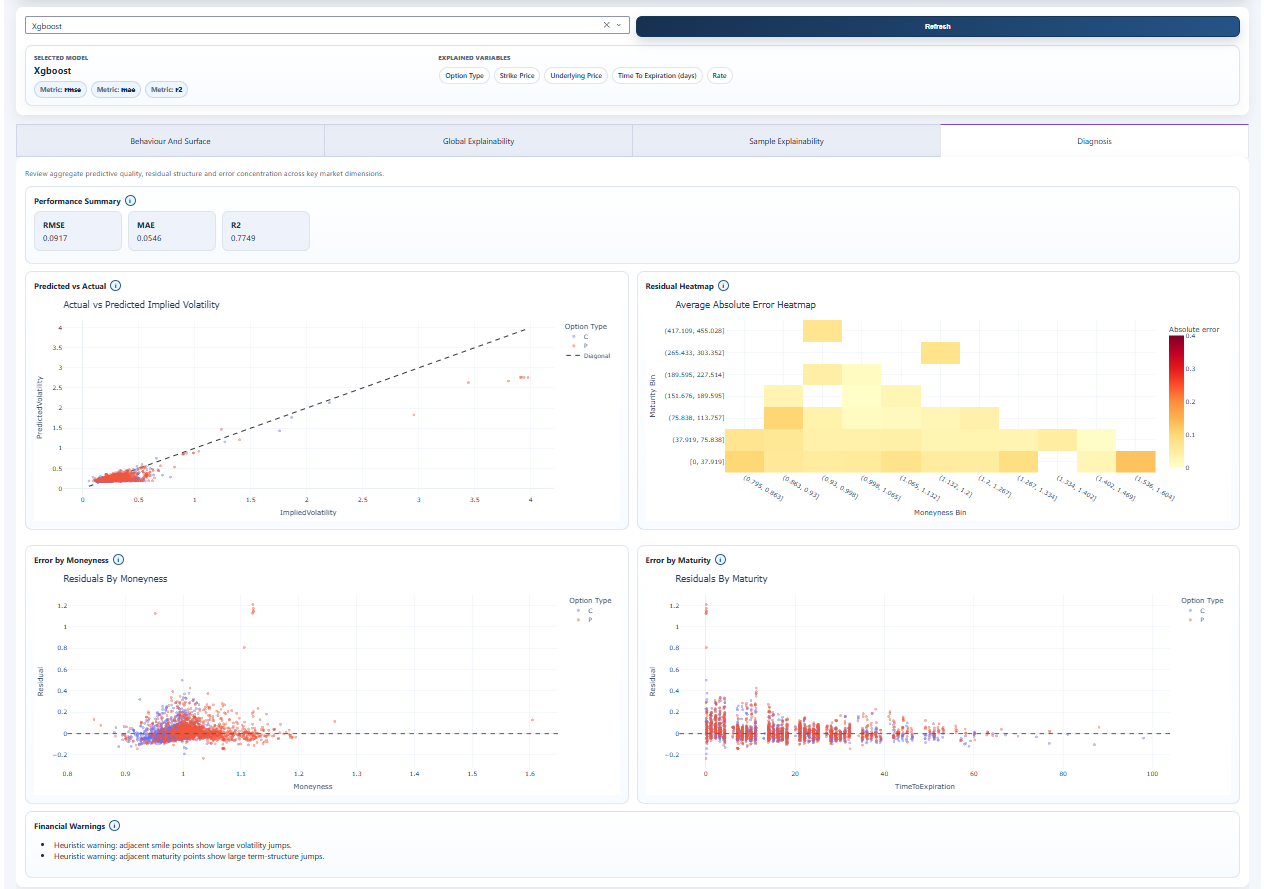
\includegraphics[width=0.8\textwidth]{imgs/dashboard/Diagnosis - Xgboost.png}
\caption{\small \emph{Diagnosis} en XGBoost.}
\label{fig:dash-diagnosis-comparison}
\end{figure}

Las vistas del dashboard son necesarias para localizar dónde aparece esa compresión. El scatter \emph{predicted vs actual} debe confirmar si los extremos altos y bajos se acercan a la media; el residual heatmap debe separar error por moneyness y vencimiento; y las cajas \emph{Error by Moneyness} y \emph{Error by Maturity} deben indicar si los extremos de moneyness o los vencimientos cortos concentran el fallo. La conclusión accionable es que el modelo es competitivo agregadamente, pero su uso debe acompañarse de diagnóstico por zonas de la superficie cuando se consulten contratos poco líquidos o alejados de ATM.



\subsubsection{Análisis del impacto del entrenamiento Progressive ATM}
\label{subsubsec:atm-impact}

El proyecto incluyó una variante experimental denominada Progressive ATM (o \emph{Entrenamiento Progresivo Ordenado por ATM}): un enfoque de aprendizaje que reordena cronológicamente el entrenamiento para presentar primero observaciones cercanas al ATM (moneyness bajo, $|\log(F/K)| < 0.05$), donde concentra la máxima liquidez y menor ruido, para después incorporar progresivamente observaciones hacia extremos de moneyness y vencimientos cortos. La motivación financiera es doble:
\begin{enumerate}
    \item La zona ATM en opciones sobre índices suele ser la más líquida y menos afectada por sesgos de selección.
    \item entrenar primero en datos menos ruidosos podría regularizar arquitecturas sensibles al orden de presentación, como redes neuronales secuenciales y modelos cuánticos inspirados.
\end{enumerate}

Complementar lectura con el Apéndice \ref{app:progressive}.


\textbf{Metodología de evaluación.} Se reentrenaron independientemente los cinco modelos de la familia de seleccionados bajo esta variante, conservando la validación cruzada 5-fold y los mismos hiperparámetros que en el entrenamiento estándar. Se compararon las métricas test de RMSE, MAE y $R^2$ entre ambas versiones (estándar vs.\ ATM) para cada familia. El análisis se complementó con inspección visual de residual heatmaps en el dashboard para verificar si la reordenación producía cambios en la distribución espacial del error (por moneyness y vencimiento).


\textbf{Síntesis interpretativa del impacto ATM por arquitectura.} Los resultados revelan un patrón sistemático: la técnica Progressive ATM no produce un modelo mejor de forma universal, sino que su efectividad depende críticamente de la arquitectura subyacente.

\begin{itemize}

    \item Modelos ya óptimos (Random Forest, y en menor medida XGBoost base): El entrenamiento progresivo ATM no mejora; en XGBoost incluso resulta perjudicial. La razón es que estos modelos ya poseen mecanismos de regularización o agregación intrínsecos (bootstrap, boosting) que no se benefician de reordenamientos externos. Forzar un orden artificial puede introducir sesgo de inicialización que degrada capacidad global de la arquitectura, particularmente en modelos iterativos como boosting.
    
    \item Modelos de baja capacidad o convergencia frágil (Sequential NN, Quantum Inspired): El entrenamiento progresivo ATM produce mejoras tangibles. Estos modelos carecen de regularización inherente y son sensibles a inicialización y orden de muestras. Entrenar primero en región ATM establece trayectoria de aprendizaje más robusta, evitando convergencia a mínimos pobres que es frecuente cuando se enfrentan datos heterogéneos desde el inicio.
    
    \item Modelos lineales (Linear Regression): El orden es irrelevante puesto que la hipótesis es global. No hay beneficio de regularización local.
    
\end{itemize}



\subsection{Behaviour And Surface}
\label{subsec:behaviour-results}

El modelo final debe leerse como función financiera, no solo como tabla de errores. Las superficies generadas alrededor de puntos de referencia del test permiten inspeccionar \(\hat{\sigma}(m,T)\), smiles y estructuras temporales.

\begin{figure}[!htbp]
\centering
\caption{\small \emph{Behaviour And Surface} de XGBoost.}
\label{fig:dash-behaviour-best-models-id1406}
\end{figure}

La lectura recomendada es usar al menos tres puntos de referencia: una observación ATM líquida, una observación en extremos de moneyness y una observación de vencimiento corto. Si el dashboard muestra saltos alrededor de un punto, la explicación debe cruzarse con vecinos y residual heatmap antes de atribuirlo a señal financiera. Si el smile es suave y el error local bajo, la predicción es más defendible.

La Figura~\ref{fig:dash-behaviour-best-models-id1406} muestra que las curvas smile y term-structure de XGBoost mantienen forma financiera interpretable (mínimo en entorno ATM y descenso de volatilidad al aumentar vencimiento para moneyness fija)



\subsection{Explicabilidad global}
\label{subsec:global-results}

La explicación global debe comprobar que los drivers principales son coherentes con la geometría de volatilidad: moneyness, vencimiento, subyacente, strike, tipo y tipo de opción. SHAP se calcula sobre variables raw visibles y el runtime reconstruye las features transformadas, por lo que una contribución de \texttt{StrikePrice} o \texttt{UnderlyingPrice} debe interpretarse en relación con moneyness y no como efecto causal aislado.

\begin{figure}[htbp]
\centering
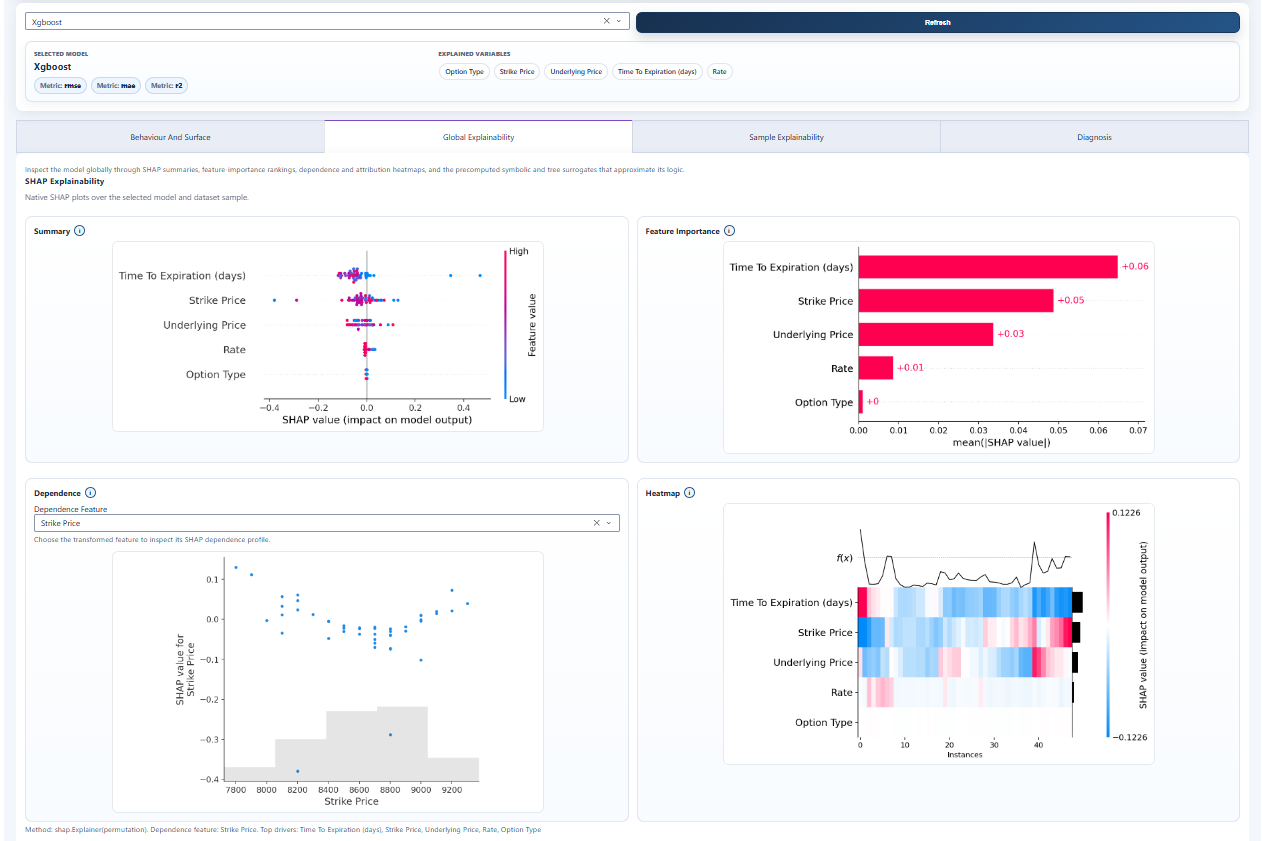
\includegraphics[width=0.8\textwidth]{imgs/dashboard/Global Explainability - Xgboost I.png}
\caption{\small SHAP global XGBoost.}
\label{fig:dash-global-shap-comparison}
\end{figure}

La lectura correcta combina ranking, signo local y dependence plots. Si una variable domina el ranking pero tiene colores mezclados o contribuciones con mucha dispersión, el modelo está usando interacciones. Esa conclusión es razonable en opciones, porque strike, subyacente y vencimiento no son independientes. Si aparecen saltos en dependence plots, deben contrastarse con las superficies y con diagnóstico por zonas de la superficie.

En las cinco variantes revisadas, y para lo que se visualiza en dashboard, la jerarquía global aparece estable: \texttt{Time To Expiration (days)} como driver principal y \texttt{Strike Price} como segundo, seguidas por \texttt{Underlying Price}; \texttt{Rate} y \texttt{Option Type} tienen peso menor. La Figura~\ref{fig:dash-global-shap-comparison} hace visible esta regularidad, que coincide con la lectura financiera esperada de superficie. El punto importante es que la consistencia entre modelos se observa en el orden de importancia, no necesariamente en la magnitud de impacto: Quantum Inspired y Sequential NN muestran dispersión SHAP más amplia para algunos rangos, coherente con su mayor sensibilidad local en otras pestañas.



\subsection{Modelos equivalentes: árboles y regresión simbólica}
\label{subsec:equivalent-results}

\begin{figure}[htbp]
    \centering
    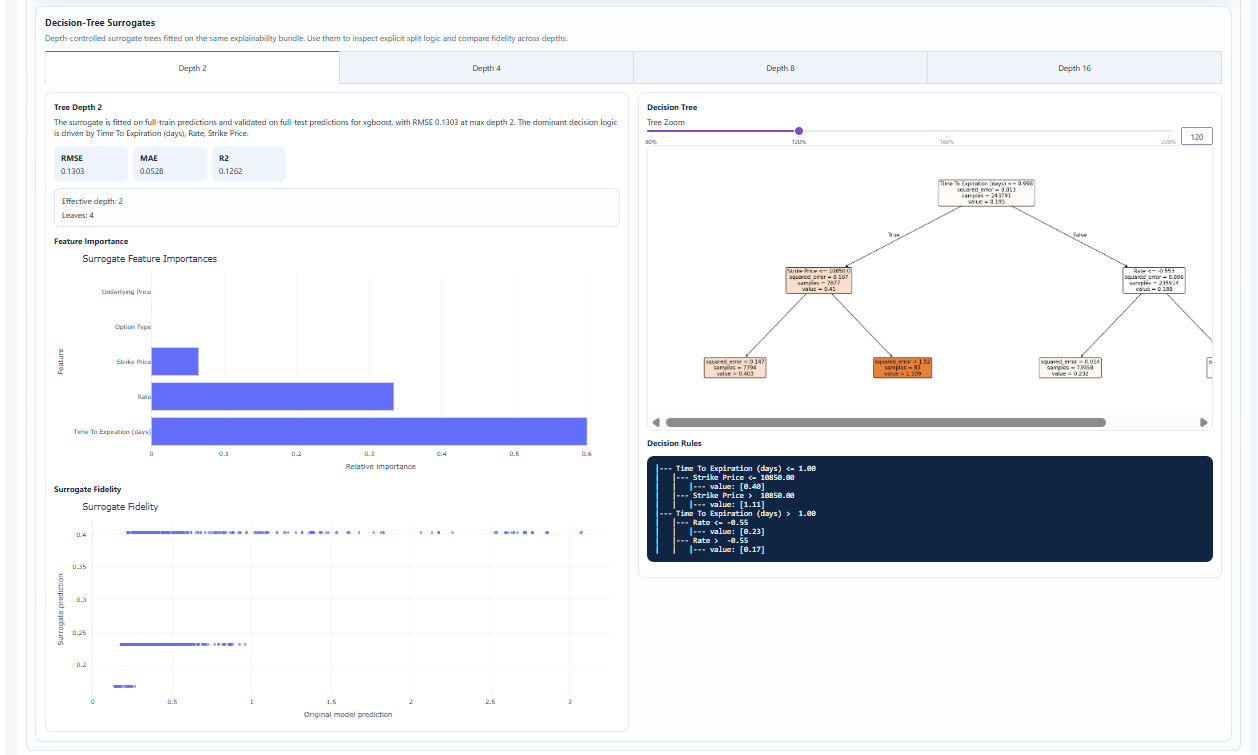
\includegraphics[width=0.8\textwidth]{imgs/dashboard/Global Explainability - Xgboost III.png}
    \caption{\small Árboles surrogate por profundidad en  XGBoost.}
    \label{fig:dash-tree-depth-rf-vs-xgb}
\end{figure}

\begin{table}[htbp]
    \centering
    \small
    \begin{tabular}{lrrr}
    \toprule
    Modelo & RMSE simbólico & MAE simbólico & \(R^2\) simbólico \\
    \midrule
    Regresión lineal & 0.0244 & 0.0135 & 0.7585 \\
    Quantum Inspired NN & inf & inf & inf \\
    Random Forest & 339.9547 & 3.5845 & -5,173,729.5872 \\
    Sequential NN & 0.0376 & 0.0316 & 0.8890 \\
    XGBoost & 0.0378 & 0.0219 & 0.9264 \\
    \bottomrule
    \end{tabular}
    \caption{Fidelidad de regresión simbólica reportada en dashboard por familia de modelo.}
    \label{tab:symbolic-fidelity-all-models}
\end{table}

Los modelos equivalentes explican el predictor, no la verdad de mercado. Para Random Forest, las métricas de fidelidad de árboles surrogate son:

\begin{table}[htbp]
\centering
\small
\begin{tabular}{rrrr}
\toprule
Profundidad & RMSE fidelidad & MAE fidelidad & \(R^2\) fidelidad \\
\midrule
2 & 0.139477 & 0.053488 & 0.129099 \\
4 & 0.135217 & 0.050783 & 0.181486 \\
8 & 0.141899 & 0.058392 & 0.098593 \\
16 & 0.144616 & 0.053187 & 0.063747 \\
\bottomrule
\end{tabular}
\caption{Fidelidad de árboles surrogate frente al Random Forest seleccionado.}
\label{tab:surrogate-rf}
\end{table}

La fidelidad de los árboles es limitada: ni siquiera profundidades altas reproducen bien el comportamiento completo del XGBoost. Esto no invalida el modelo principal, pero sí limita el uso de reglas simples como explicación global. La regresión simbólica (ver Tabla \ref{tab:surrogate-rf}) generada para este paquete muestra métricas no utilizables para defensa del Random Forest ni del Quantum Inspired NN, con RMSE de fidelidad extremadamente alto; por tanto, el modelo más fiable que obtenemos es el XGBoost.

La Figura~\ref{fig:dash-tree-depth-rf-vs-xgb}, junto con la Tabla~\ref{tab:surrogate-rf} y la Tabla~\ref{tab:symbolic-fidelity-all-models}, permite una conclusión transversal: la facilidad para explicar un modelo mediante reglas o fórmulas compactas no coincide necesariamente con su capacidad predictiva final en test.


\subsection{Explicabilidad local y soporte histórico}
\label{subsec:local-results}

El análisis local debe seleccionar una muestra representativa y una muestra problemática. Para cada una, el waterfall SHAP explica la predicción como suma de valor base y contribuciones. Los vecinos históricos, calculados contra train en el espacio transformado y estandarizado, indican si la muestra está dentro de una región conocida. En el paquete se guardan hasta 200 vecinos por muestra, usando una referencia de entrenamiento de hasta 20.000 observaciones.

\begin{figure}[htbp]
\centering
\begin{minipage}{0.49\textwidth}
\centering
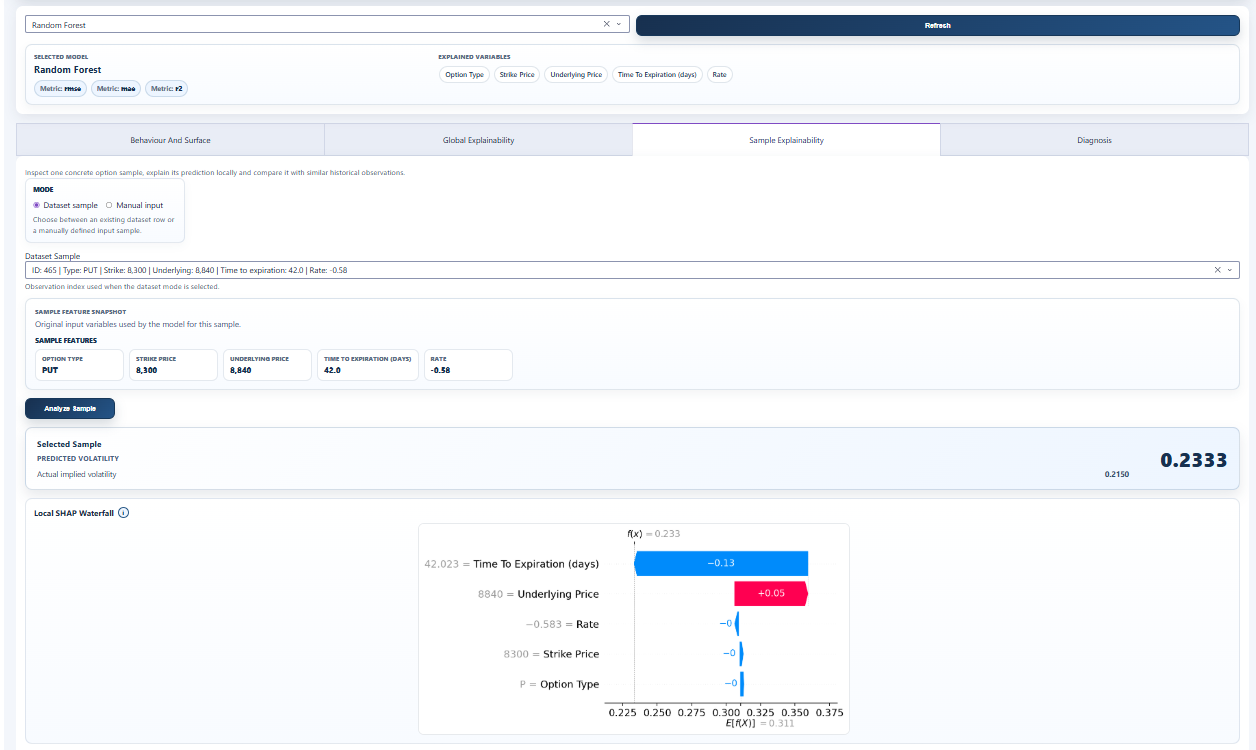
\includegraphics[width=\textwidth,height=0.23\textheight,keepaspectratio]{../imgs/dashboard/Sample Explainability - Random Forest I.png}
\end{minipage}\hfill
\begin{minipage}{0.49\textwidth}
\centering
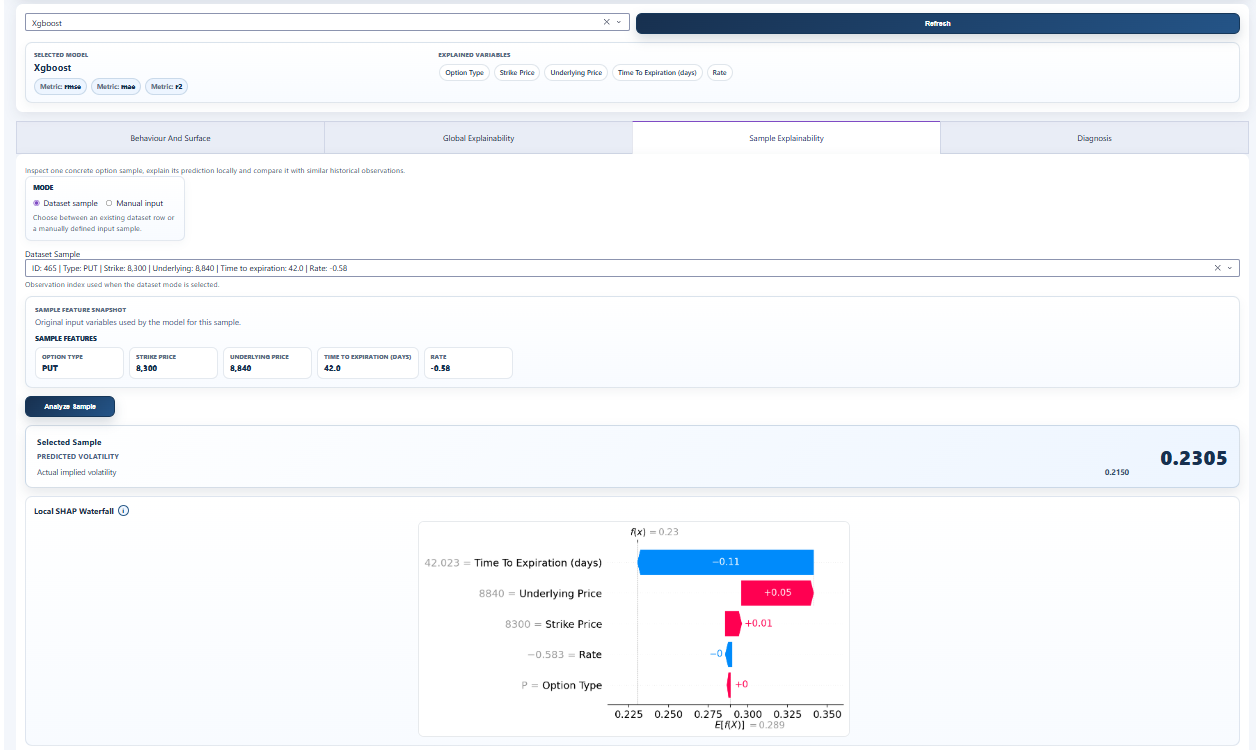
\includegraphics[width=\textwidth,height=0.23\textheight,keepaspectratio]{../imgs/dashboard/Sample Explainability - Xgboost I.png}
\end{minipage}
\caption{\small Explicabilidad local en modo \emph{dataset} para la misma muestra (ID 465): comparación Random Forest vs XGBoost.}
\label{fig:dash-local-dataset-rf-xgb}
\end{figure}

\begin{figure}[htbp]
\centering
\begin{minipage}{0.49\textwidth}
\centering
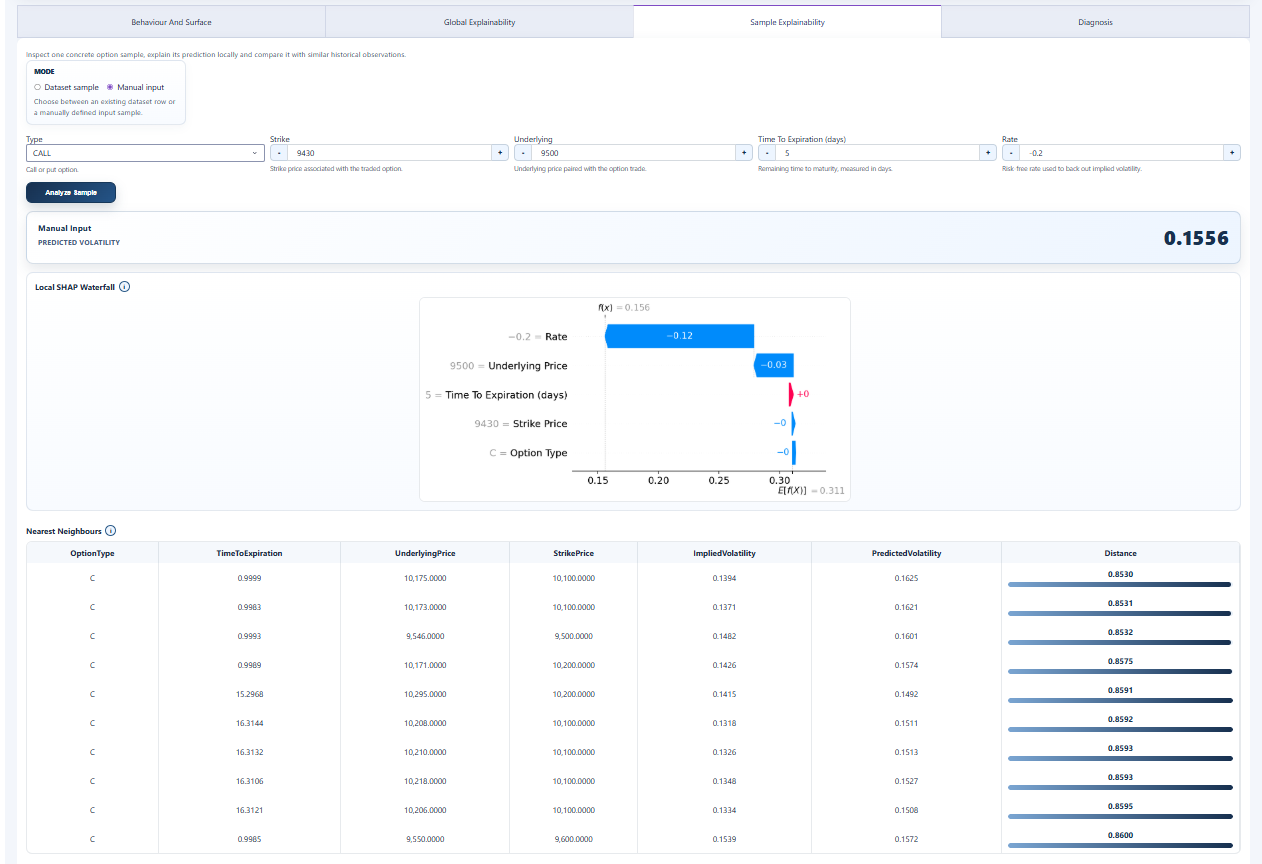
\includegraphics[width=\textwidth,height=0.23\textheight,keepaspectratio]{../imgs/dashboard/Sample Explainability - Random Forest III.png}
\end{minipage}\hfill
\begin{minipage}{0.49\textwidth}
\centering
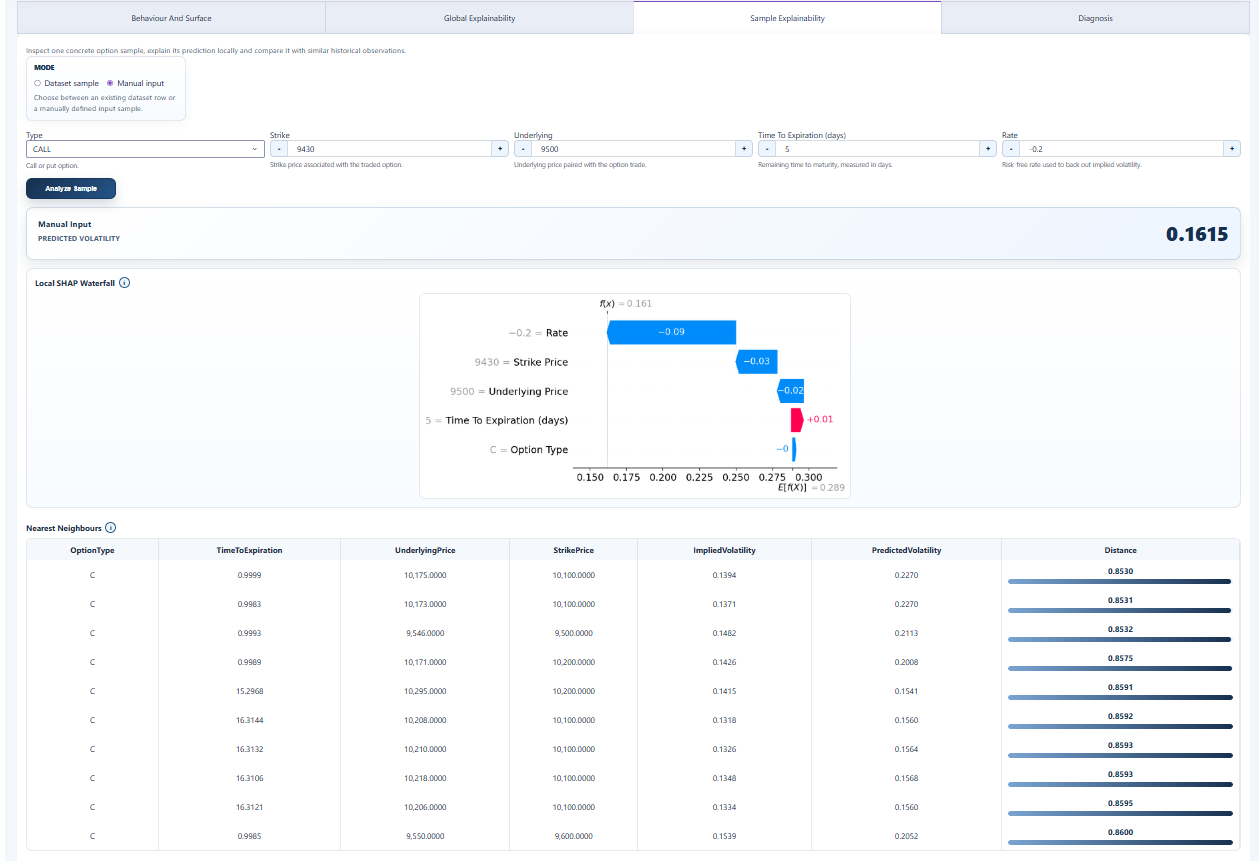
\includegraphics[width=\textwidth,height=0.23\textheight,keepaspectratio]{../imgs/dashboard/Sample Explainability - Xgboost III.png}
\end{minipage}
\caption{\small Explicabilidad local en modo \emph{manual input} (stress corto vencimiento): contraste de coherencia local y soporte histórico en ambos finalistas.}
\label{fig:dash-local-manual-rf-xgb}
\end{figure}

La interpretación profesional debe combinar ambas piezas. Si una muestra tiene waterfall coherente y vecinos cercanos con volatilidades similares, la explicación es sólida. Si el waterfall parece razonable pero los vecinos están lejos, el modelo puede estar extrapolando; en ese caso, la predicción debe revisarse con diagnóstico por zonas de la superficie y superficie local.

El contraste entre Figuras~\ref{fig:dash-local-dataset-rf-xgb} y~\ref{fig:dash-local-manual-rf-xgb} muestra una coherencia especialmente relevante para defensa técnica. En la muestra real (ID 465), Random Forest y XGBoost predicen prácticamente el mismo nivel (\(\sim 0.233\) y \(\sim 0.231\)), con waterfall de signo consistente: \texttt{Time To Expiration} aporta caída y \texttt{Underlying Price} compensa parcialmente al alza, en línea con su papel dominante en SHAP global. En el caso manual de vencimiento corto, ambos modelos reducen volatilidad prevista respecto al valor base y, al mismo tiempo, los vecinos aparecen a distancia alta (\(\sim 0.85\)), señalando un escenario de menor soporte histórico. Esta combinación (coherencia de mecanismo + menor densidad local) justifica usar la explicación local como guía de prudencia, no como validación automática de calidad de mercado.

\textbf{Como regla práctica, una explicación local es más defendible cuando se cumplen tres condiciones.}

\begin{itemize}
  \item El signo y magnitud de las contribuciones SHAP son compatibles con la intuición financiera del caso.
  \item Los vecinos cercanos muestran contratos, moneyness y vencimientos realmente parecidos.
  \item El error por zonas del modelo no es anómalamente alto en esa área.
\end{itemize}

Cuando falla alguna de esas tres condiciones, la lectura debe cambiar: la explicación sigue diciendo cómo razona el modelo, pero deja de ser una justificación sólida de que la predicción sea fiable en términos de mercado.

\subsection{Síntesis comparativa por temática}
\label{subsec:sintesis-tematica-modelos}

Para cerrar la lectura de dashboard con una vista única y defendible, la Tabla~\ref{tab:sintesis-tematica-modelos} resume las conclusiones cualitativas por temática (filas) y por familia de modelo (columnas). Esta síntesis se apoya en las capturas de diagnóstico, comportamiento, explicabilidad global/local y modelos equivalentes revisadas en esta sección.

\begin{table}[htbp]
\centering
\small
\begin{adjustbox}{max width=\textwidth}
\begin{tabular}{p{0.24\textwidth}p{0.14\textwidth}p{0.14\textwidth}p{0.14\textwidth}p{0.14\textwidth}p{0.14\textwidth}}
\toprule
Temática & Reg. lineal & Random Forest & XGBoost & Sequential NN & Quantum Inspired \\
\midrule
Driver SHAP dominante & TTE (muy dominante) & TTE (estable) & TTE (estable) & TTE (estable) & TTE (estable) \\

Segundo driver global & Strike (alto) & Strike (alto) & Strike (alto) & Strike (medio) & Strike (medio) \\

Rendimiento diagnóstico test & Bajo & Alto (mejor) & Alto (2º) & Medio-bajo & Bajo \\

Suavidad de superficie local & Alta (simple) & Media (escalones locales) & Media (escalones locales) & Media-baja & Media-baja \\

Patrón smile/skew en ICE-ALE & Visible, menos rico & Visible y consistente & Visible y consistente & Visible, más inestable & Visible, más inestable \\

Coherencia Global \textrightarrow{} Sample & Media & Alta & Alta & Media & Media \\

Soporte histórico en casos manuales exigentes & N/A en muestra principal & Distancia alta en estrés corto T & Distancia alta en estrés corto T & N/A en muestra principal & N/A en muestra principal \\

Compresibilidad en modelo equivalente (simbólico/árbol) & Alta (simple) & Muy baja (no compactable) & Media-alta & Media-alta & Muy baja/No utilizable \\
\bottomrule
\end{tabular}
\end{adjustbox}
\caption{Síntesis de conclusiones por temática y por familia de modelo a partir de lo visualizado en el dashboard. TTE: \texttt{Time To Expiration}.}
\label{tab:sintesis-tematica-modelos}
\end{table}

Esta síntesis permite sostener dos mensajes, con alcance observacional sobre lo visualizado en el dashboard. Primero, la estructura explicativa principal aparece consistente entre familias: el vencimiento domina y el strike ocupa una posición secundaria relevante, coherente con la geometría de superficie. Segundo, las diferencias clave entre modelos no están tanto en qué variables miran, sino en cómo transforman esa información en estabilidad local, error por zonas y facilidad de explicación compacta. Para afirmar universalidad sobre todos los trades sería necesario un contraste estadístico adicional fuera de las muestras visualizadas.

\section{Aplicaciones operativas y validación independiente}
\label{sec:aplicaciones-operativas}

Este apartado conecta los resultados del dashboard con usos profesionales concretos en valoración, control de riesgos y gobierno de modelos. El objetivo no es extrapolar más allá de la evidencia disponible, sino traducir lo observado en reglas de uso defendibles para un entorno de mesa y model validation. El detalle visual de sensibilidad por regiones se amplía en el Anexo~\ref{app:sensibilidad-moneyness-vencimiento}.

\subsection{Validación independiente de modelos internos}
\label{subsec:validacion-independiente}

El modelo final puede utilizarse como referencia independiente para contrastar superficies internas de valoración. En la práctica, la validación no se limita a comparar un único precio, sino que contrasta consistencia por regiones de moneyness y vencimiento. Un desacople localizado entre el pricer interno y la referencia empírica puede señalar problemas de parametrización, de datos de entrada o de régimen de mercado no recogido por el enfoque clásico.

\begin{itemize}
  \item \textbf{Nivel agregado:} contraste de RMSE/MAE y de dispersión global frente a un benchmark interno.
  \item \textbf{Nivel por superficie:} contraste de residual heatmap y cajas de error por moneyness/vencimiento para detectar discrepancias localizadas.
  \item \textbf{Nivel de caso:} uso de SHAP local y vecinos para justificar por qué una diferencia concreta es esperable o requiere revisión.
\end{itemize}

Este enfoque es especialmente útil cuando el área de validación necesita una segunda opinión cuantitativa que no comparta la misma familia paramétrica que el modelo interno de producción.

\subsection{Interpolación y suavizado: alcance real del enfoque}
\label{subsec:interpolacion-suavizado-alcance}

Conviene precisar el alcance metodológico. En este trabajo no se impone una interpolación paramétrica cerrada de la superficie (por ejemplo, una sola fórmula global calibrada ex ante). La superficie se aprende de forma empírica a partir de observaciones de mercado mediante modelos supervisados. Por tanto, la ``interpolación'' se produce de forma implícita a través de la función aprendida $\hat{\sigma}(m,T,\dots)$ y se evalúa visualmente con las vistas de \emph{Behaviour And Surface} y \emph{Diagnosis}.

La suavidad no se da por supuesta: se verifica. Si aparecen escalones locales o concentraciones de error en zonas concretas, el resultado se interpreta como limitación del modelo en esa región, no como propiedad financiera del mercado. Esta distinción es clave para no confundir capacidad predictiva local con una estructura de superficie económicamente robusta.

\subsection{Detección de anomalías de precio y errores de mercado}
\label{subsec:anomalias-precio-mercado}

La detección de anomalías se construye en dos capas complementarias. La primera está en el ETL, con controles de calidad (precios y cantidades válidas, coherencia temporal opción-subyacente, resolución numérica estable de volatilidad implícita). La segunda está en diagnóstico ex post, donde los residuales por zona de superficie permiten localizar trades atípicos en extremos de moneyness o vencimientos cortos.

En términos operativos, una anomalía no se define sólo por error alto puntual, sino por contexto: error alto junto con baja densidad de vecinos, geometría local inestable o incoherencia entre explicación local y patrón global. Esta lectura reduce falsos positivos y mejora la utilidad del modelo como filtro de revisión manual.

\subsection{Valoración de ilíquidas, control de mesa, auditoría y cobertura}
\label{subsec:uso-operativo-derivados}

Las aplicaciones más exigentes se apoyan en la misma secuencia de lectura: diagnóstico por zonas, contraste funcional de superficie y justificación local. Con ese flujo, el modelo aporta soporte en cuatro frentes conectados:

\begin{itemize}
  \item \textbf{Valoración de opciones ilíquidas o poco negociadas:} cuando no hay suficiente señal transaccional directa, la predicción basada en superficie y vecinos históricos ofrece una referencia empírica utilizable, con cautela reforzada en extremos.
  \item \textbf{Control de riesgos de mesa de derivados:} la lectura por moneyness y vencimiento permite identificar dónde el error puede contaminar griegas, escenarios o límites de riesgo más que la media global.
  \item \textbf{Explicación ante auditoría interna/model validation:} SHAP global/local, trazabilidad de pipeline y evidencias por superficie permiten defender decisiones de modelo con base reproducible.
  \item \textbf{Soporte a decisiones de cobertura:} la geometría smile/term-structure más el diagnóstico local aportan contexto para priorizar coberturas en zonas de mayor sensibilidad o menor soporte histórico.
\end{itemize}

La conclusión práctica es que el modelo no sustituye el juicio de mercado, pero sí mejora su calidad: convierte decisiones difíciles en decisiones mejor informadas, trazables y auditables.

\section{Discusión}
\label{sec:discusion}

La pregunta planteada en \autoref{sec:planteamiento} puede responderse afirmativamente con matices. Sí es posible construir un modelo útil y consultable para volatilidad implícita de opciones del IBEX; el Random Forest seleccionado ofrece buen error en test. El matiz es que la explicación no puede descansar en un único resumen global: la fidelidad de modelos equivalentes simples es limitada, y la defensa técnica debe combinar SHAP, superficies, ICE/ALE, vecinos y diagnóstico.

\subsection{Lectura financiera}
\label{subsec:discusion-financiera}

Financieramente, el proyecto trata la volatilidad como superficie y no como serie unidimensional. El buen RMSE agregado es relevante, pero el dato más importante para gestión de riesgos es dónde se produce el error. La compresión de volatilidades extremas sugiere que deben revisarse los extremos de moneyness y los vencimientos cortos con más cuidado. Este comportamiento es plausible en derivados: esas zonas suelen tener menos liquidez, más ruido de microestructura y mayor sensibilidad al desfase entre opción y futuro subyacente.

\begin{itemize}
  \item El modelo final es útil para lectura agregada y consulta, pero no debe tratarse como atajo automático del juicio financiero en zonas extremas.
  \item La geometría de la superficie sigue siendo el criterio principal de plausibilidad: smiles, term structures y suavidad local importan tanto como el error medio.
  \item La lectura de vecinos y soporte histórico es especialmente valiosa cuando se analiza un contrato poco líquido o lejano de ATM.
\end{itemize}

En otras palabras, el trabajo refuerza una idea clásica en derivados: el resultado útil no es un único número, sino una predicción situada dentro de una estructura de superficie, de un contexto de mercado y de una evidencia histórica comparable.

También conviene subrayar una implicación práctica. Cuando el modelo se usa como apoyo a valoración o revisión manual, la pregunta correcta no es sólo si ``acierta de media'', sino si conserva lógica financiera en la zona concreta que se está consultando. Esa exigencia explica por qué el documento dedica espacio a smiles, extremos de moneyness, vencimientos cortos y soporte local, y no sólo a tablas globales de error. Esta lectura aplicada se concreta en la Sección~\ref{sec:aplicaciones-operativas} y se refuerza con el anexo de sensibilidad por regiones de superficie.

\textbf{Aportación frente a enfoques clásicos.}

La comparación con enfoques clásicos debe plantearse como complementariedad y mejora operativa, no como sustitución automática. Los enfoques paramétricos (por ejemplo, parametrizaciones estáticas de superficie o ajustes locales ad hoc) aportan estructura financiera explícita y son valiosos para gobernanza. La propuesta de este TFM añade valor en escenarios donde esa estructura no basta por sí sola:

\begin{itemize}
  \item \textbf{Mayor flexibilidad empírica:} captura interacciones no lineales entre moneyness, vencimiento, subyacente y tipo con menor rigidez funcional.
  \item \textbf{Mejor lectura por zonas:} añade diagnóstico de error por región de superficie, clave para contratos ilíquidos o extremos de moneyness.
  \item \textbf{Capacidad de control y auditoría:} incorpora trazabilidad y explicaciones locales/globales en el mismo flujo de servicio.
  \item \textbf{Validación cruzada de pricing:} permite contrastar salidas de modelos clásicos internos con una referencia empírica independiente.
\end{itemize}

En términos prácticos, la mejora no es sólo bajar una métrica agregada. La mejora principal es disponer de una \emph{superficie utilizable}: consultable, explicable y controlable en producción, especialmente en los casos donde las reglas clásicas requieren juicio manual intensivo.

\subsection{Lectura de IA y Data Science}
\label{subsec:discusion-ia}

Desde la perspectiva de IA, la comparación muestra que modelos tabulares de árboles son más adecuados que redes densas para esta muestra. Random Forest y XGBoost aprovechan interacciones no lineales sin exigir escalado y ofrecen mejor test. La métrica CE\(_2\) favorece a XGBoost en train/validation, pero el test favorece a Random Forest; esto ilustra por qué la selección final no debe quedarse en validación. Progressive ATM mejora Quantum Inspired, pero no a las familias que ya generalizan mejor.

\begin{itemize}
  \item La validación temporal es más importante que una mejora marginal en entrenamiento.
  \item La estabilidad entre train, validation y test pesa más que una única métrica brillante en una fase intermedia.
  \item La explicabilidad posterior también importa: un modelo competitivo pero imposible de leer exige más apoyos y más cautela en su defensa.
\end{itemize}

Desde esta perspectiva, el trabajo también deja una lección de alcance más general: en datos financieros tabulares, una arquitectura más compleja no merece preferencia por defecto. Primero debe demostrar que generaliza mejor; después, que esa mejora compensa el coste extra de explicación, mantenimiento y servicio.

\subsection{Lectura de ingeniería y cloud}
\label{subsec:discusion-cloud}

La dimensión cloud aporta valor porque no se usa como adorno: resuelve almacenamiento, carga de modelos, despliegue independiente de API y dashboard y trazabilidad. La separación entre modelo, paquete explicativo, API, dashboard y almacenamiento reduce acoplamientos y facilita auditoría. La principal cautela operativa es mantener sincronizados modelo, scaler, metadatos y componentes explicativos; de lo contrario, el sistema podría predecir con una versión y explicar con otra.

\begin{itemize}
  \item El almacenamiento centralizado evita duplicidades manuales y facilita compartir la misma versión entre servicios.
  \item El despliegue desacoplado permite que un problema en dashboard no bloquee necesariamente la API, y viceversa.
  \item La reproducibilidad de infraestructura es útil sólo si el pipeline mantiene coherencia entre modelo servido y explicaciones persistidas.
\end{itemize}

La consecuencia práctica es que la ingeniería no aparece aquí como una capa secundaria. Es parte del argumento de calidad del trabajo: un modelo que no puede versionarse, servirse y auditarse con coherencia pierde valor aunque su ajuste estadístico sea aceptable.

\subsection{Limitaciones}
\label{subsec:limitaciones}

Las limitaciones se agrupan en cuatro bloques. Primero, la volatilidad implícita depende de la calidad del enlace opción-subyacente y del solver Black-76. Segundo, el conjunto de datos es heterogéneo en liquidez y cobertura de moneyness/vencimiento, por lo que los extremos deben diagnosticarse localmente. Tercero, la explicabilidad aproxima comportamientos del modelo y no sustituye validación económica. Cuarto, el despliegue cloud exige disciplina de versionado para evitar inconsistencias entre modelos, paquetes de dashboard y metadatos.

\begin{itemize}
  \item No toda región del espacio de entrada tiene la misma densidad histórica ni la misma calidad de soporte.
  \item Un modelo explicable sigue pudiendo estar equivocado si aprende sesgos sistemáticos de los datos.
  \item Las visualizaciones ayudan a detectar problemas, pero no convierten por sí solas una predicción en económicamente válida.
\end{itemize}

Además, hay una limitación estructural que conviene dejar explícita: el proyecto explica muy bien cómo razona el modelo entrenado, pero no agota por sí solo la validación económica del mercado. Siempre queda margen para contrastar con enfoques paramétricos, con criterios de liquidez más finos o con reglas de suavidad impuestas ex ante sobre la superficie.




